\app~is a high-efficient root cause localization approach for availability issues.
An availability issue is usually detected from the business perspective, e.g., the decline of successful orders.
It may be caused by different types of anomalies.
Currently \app~supports three types of anomalies, i.e., performance anomaly, reliability anomaly, and traffic anomaly.
When handling a specific type of anomalies, \app~considers a corresponding service call metric and a specific direction of anomaly propagation.
For example, when handling performance anomaly anomalies, \app~considers response time of service calls and the anomaly propagation direction from downstream to upstream.

\begin{figure}[ht]
	\centering
	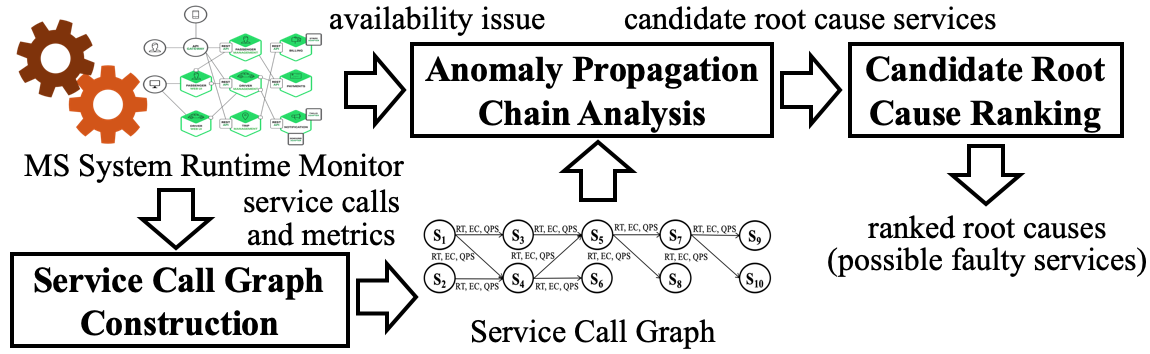
\includegraphics[width=0.5\textwidth]{images/overview.png}
	\vspace{-8pt}
	\caption{\app~Overview}\label{fig:overview}
	\vspace{-3pt}
\end{figure}

An overview of \app~is presented in Figure~\ref{fig:overview}.
The approach includes the following three parts.

\textbf{1) Service Call Graph Construction}

When the runtime monitor detects an availability issue, \app~starts a root cause analysis process.
It constructs a service call graph of the target microservice system based on the service calls and metrics captured by the runtime monitor.
The service call graph provides an updated snapshot of the microservice system by recording the service calls occurring in a latest time window (e.g., the last 30 minutes).
To facilitate the root cause analysis of availability issues, the service call graph also records various quality metrics of service calls, such as response time (RT), error count (EC), and queries per second (QPS).

%\app~ constructs and updates a service call graph of the target microservice system to represent the anomaly propagation in the system.
%As shown in Figure \ref{fig:overview}, our call graph consists of
A service call graph consists a set of service nodes S =  $\left\{ S_{1},S_{2},...,S_{n} \right\}$.
A node represents a service that is called in the latest time window (e.g., the last 30 minutes).
Note that a service may have many instances in the running system.
An edge $S_i \rightarrow S_j$ represents a service call from $S_{i}$ to $S_{j}$ that occurs in the latest time window.
For each service call, the graph records a series of values for different quality metrics (e.g., RT, EC, QPS) in the latest time window (e.g., the last 60 minutes).
For example, for each service call the graph records 60 RT values, each indicating the average response time of a minute.

The monitoring data (including service calls and their metrics) is stored in a time series database (TSDB).
When an availability issue is raised, \app~dynamically constructs a service call graph based on the data.
Services and service calls in the graph are aggregated from service instances and calls between them.
The metrics of a service call $S_i \rightarrow S_j$ are also aggregated from the corresponding metrics of the calls from the instances of $S_i$ to those of $S_j$.
It uses Flink~\cite{flink}, a distributed streaming data-flow engine, to aggregate the data.
To optimize the performance, the service call graph is constructed in an on-demand and incremental way with the anomaly propagation chain analysis process:
only when a service call is reached in the analysis the data about it is pulled from the TSDB.

\textbf{2) Anomaly Propagation Chain Analysis}

An availability issue is initially reported on a service (called \textit{initial anomalous service}), but the root cause often lies in some of its downstream or upstream services.
A root cause service and an initial anomalous service are usually connected by an anomaly propagation chain composed of a series of anomalous services.
The purpose of anomaly propagation chain analysis is to identify a set of candidate root cause services by analyzing possible anomaly propagation chains from the initial anomalous service.

Based on the service call graph, \app~analyzes possible anomaly propagation chains from the initial anomalous service of the availability issue.
%To this end, it traverses the service call graph along anomalous service call edges detected based on service call metrics.
The analysis is done by traversing the service call graph along anomalous service call edges, starting from the initial anomalous service and following the opposite directions of possible anomaly propagation directions.
Each anomaly propagation chain considers a specific anomaly type propagated from a neighboring service of the initial anomalous service.
To improve the efficiency, \app~adopts a pruning strategy to eliminate anomalous service call edges that are irrelevant to the current anomaly propagation chain.
This anomaly propagation chain analysis ends with a set of services as candidate root causes, each associated with a specific anomaly type.
The analysis process together with the service anomaly detection method and the pruning strategy are detailed in Section~\ref{sec:propagation}.

\textbf{3) Candidate Root Cause Ranking}

%The anomaly propagation chain analysis usually results in several to dozens of candidate root causes.
%As the verification of candidate root causes is time-consuming, the developers usually do not want to
\app~ranks candidate root causes based on the possibility of causing the given availability issue.
Based on our analysis of the monitoring data, we find that the anomaly index of the initial anomalous service has similar change trends with the anomaly index of the root cause service.
Note that the anomaly index of the initial anomalous service is some kind of business metric (e.g., number of successful orders), while the anomaly index of a candidate root cause is some kind of quality metric (e.g., RT, EC, QPS).
Therefore, we use the Pearson correlation coefficient~\cite{perlationcorrelation} to measure the similarity of the change trends of the two anomaly indexes and rank the candidate root causes by the correlation coefficient.

For the initial anomalous service, the service call graph records a business metric value (e.g., number of successful orders) per minute.
For a candidate root cause service, the service call graph records a value for the quality metric (e.g., RT, EC, QPS) of the corresponding anomaly type per minute.
To reflect the latest change trends, we only consider the metric values in a latest time window (e.g., the last 60 minutes).
The values for a specific business metric of the initial anomalous service in the last $n$ minutes thus can be represented by a vector $X$, where $X_i$ ($1 \leq i \leq n$) represents the value of the $i$th minute.
Similarly, the values for a specific quality metric of a candidate root cause service in the last $n$ minutes can be represented by a vector $Y$.
Their Pearson correlation coefficient can be calculated as Equation~\ref{eq:pearson}, where $\bar{X}$ and $\bar{Y}$ represent the average of $X$ and $Y$ respectively.
%And take the absolute value P(XY) of the correlation coefficient for the reason that the positive and negative correlation exist in the anomaly propagation in cloud native systems~\cite{DCCGRID2018CloudRange}.
A positive (negative) value of $P(X, Y)$ indicates a positive (negative) correlation; and the larger the absolute value of $P(X, Y)$ (i.e., $|P(X, Y)|$), the more likely that the two change trends correlate.
Therefore, we rank the candidate root causes by the absolute value of the Pearson correlation coefficient.

\begin{equation}
\label{eq:pearson}
P(X, Y) =  \frac{ \sum_{i=1}^{n} (X_i -\bar{X})(Y_i - \bar{Y})  )}{\sqrt{\sum_{i=1}^{n} (X_i - \bar{X})^2\sum_{i=1}^{n} (Y_i - \bar{Y})^2}}
\end{equation}



%We detail the three phases of \app, i.e., service call graph construction, anomaly propagation chain analysis, candidate root cause ranking, in Section~\ref{sec:callgraph}, \ref{sec:chain}, \ref{sec:ranking}, respectively.
%A key in anomaly propagation chain analysis is the anomaly detection of individual services, so we also detail service anomaly detection in Section~\ref{sec:anomaly}.

